\documentclass[a4paper, 12pt]{article}
\usepackage{pgfplots, mathtools}

%% Listings With Code-Styling and Grey Background
\usepackage{float, listings} 
\lstset{						% Global Listing settings
	language=Verilog,
	numbers=left,
	numberstyle=\tiny\color{gray},
%	firstnumber=1,
	numberfirstline=true,
	stepnumber=1,
	tabsize=2,
	breaklines=true,
}
\usepackage{xcolor, mdframed, graphicx}
\definecolor{code-gray}{gray}{0.93}

%% Make specific pages landscale for larger figures
\usepackage{pdflscape}

%% Custom FSM's
\usepackage{tikz}
\usetikzlibrary{automata, positioning, arrows, positioning}
\tikzset{very thick, ->, >=stealth', node distance=6cm, every state/.style={thick, fill=gray!10}, initial text=$ $}

%% Automatic Word Formatting
\usepackage{xspace}
\newcommand*{\Vivado}{\textit{Vivado}\xspace} % Italicize Vivado
\newcommand*{\SV}{\textbf{SystemVerilog}\xspace} % Bold SystemVerilog

%% Clickable links in the output PDF
\usepackage{hyperref}
\hypersetup{colorlinks=true, linktoc=all, linkcolor=black}

%% Figure Numbering Within Sections
\let\counterwithout\relax
\let\counterwithin\relax
\usepackage{chngcntr}
\counterwithin{figure}{section}

%% Macros for logic timing diagrams
\newcounter{wavenum}
\setlength{\unitlength}{1cm}
% advance clock one cycle, not to be called directly
\newcommand*{\clki}{
  \draw (t_cur) -- ++(0,.3) -- ++(.5,0) -- ++(0,-.6) -- ++(.5,0) -- ++(0,.3)
    node[time] (t_cur) {};
}
\newcommand*{\bitvector}[3]{
  \draw[fill=#3] (t_cur) -- ++( .1, .3) -- ++(#2-.2,0) -- ++(.1, -.3)
                         -- ++(-.1,-.3) -- ++(.2-#2,0) -- cycle;
  \path (t_cur) -- node[anchor=mid] {#1} ++(#2,0) node[time] (t_cur) {};
}
% \known{val}{length}
\newcommand*{\known}[2]{
    \bitvector{#1}{#2}{white}
}
% \unknown{length}
\newcommand*{\unknown}[2][XXX]{
    \bitvector{#1}{#2}{black!20}
}
% \bit{1 or 0}{length}
\newcommand*{\bit}[2]{
  \draw (t_cur) -- ++(0,.6*#1-.3) -- ++(#2,0) -- ++(0,.3-.6*#1)
    node[time] (t_cur) {};
}
% \unknownbit{length}
\newcommand*{\unknownbit}[1]{
  \draw[ultra thick,black!50] (t_cur) -- ++(#1,0) node[time] (t_cur) {};
}
% \nextwave{name}
\newcommand{\nextwave}[1]{
  \path (0,\value{wavenum}) node[left] {#1} node[time] (t_cur) {};
  \addtocounter{wavenum}{-1}
}
% \clk{name}{period}
\newcommand{\clk}[2]{
    \nextwave{#1}
    \FPeval{\res}{(\wavewidth+1)/#2}
    \FPeval{\reshalf}{#2/2}
    \foreach \t in {1,2,...,\res}{
        \bit{\reshalf}{1}
        \bit{\reshalf}{0}
    }
}

% \begin{wave}[clkname]{num_waves}{clock_cycles}
\newenvironment{wave}[3][clk]{
  \begin{tikzpicture}[draw=black, yscale=.7,xscale=1]
    \tikzstyle{time}=[coordinate]
    \setlength{\unitlength}{1cm}
    \def\wavewidth{#3}
    \setcounter{wavenum}{0}
    \nextwave{#1}
    \foreach \t in {0,1,...,\wavewidth}{
      \draw[dotted] (t_cur) +(0,.5) node[above] {t=\t} -- ++(0,.4-#2);
      \clki
    }
}{\end{tikzpicture}}

%$ Specific Line Breaks
% See https://tex.stackexchange.com/questions/26174/ for details
\usepackage[british]{babel} 

%% Page Margins
\usepackage[margin=1.00in]{geometry}

%% Beginning of Document
\begin{document}
\counterwithin{lstlisting}{section} % Listings are numbered within sections
% Title
\title{ECE 440 - Project \#5}
\author{Collin Heist}
\date{\today}
\maketitle

% Table of Content and Listings
\pagenumbering{roman}
\tableofcontents
\renewcommand{\listfigurename}{Figures}
\listoffigures
\lstlistoflistings
\newpage
\pagenumbering{arabic}

% Beginning of Report
\section{Design}
\subsection{Top-Level Module}
To start the design process, I created my top-level \textit{memory reading} module. This module interacts with all pieces of the design (except the debounce circuitry); including the block memory, GCD calculator, and the SPI module. The FSM I ended up implementing was the following:

\begin{figure}[H]
\centering
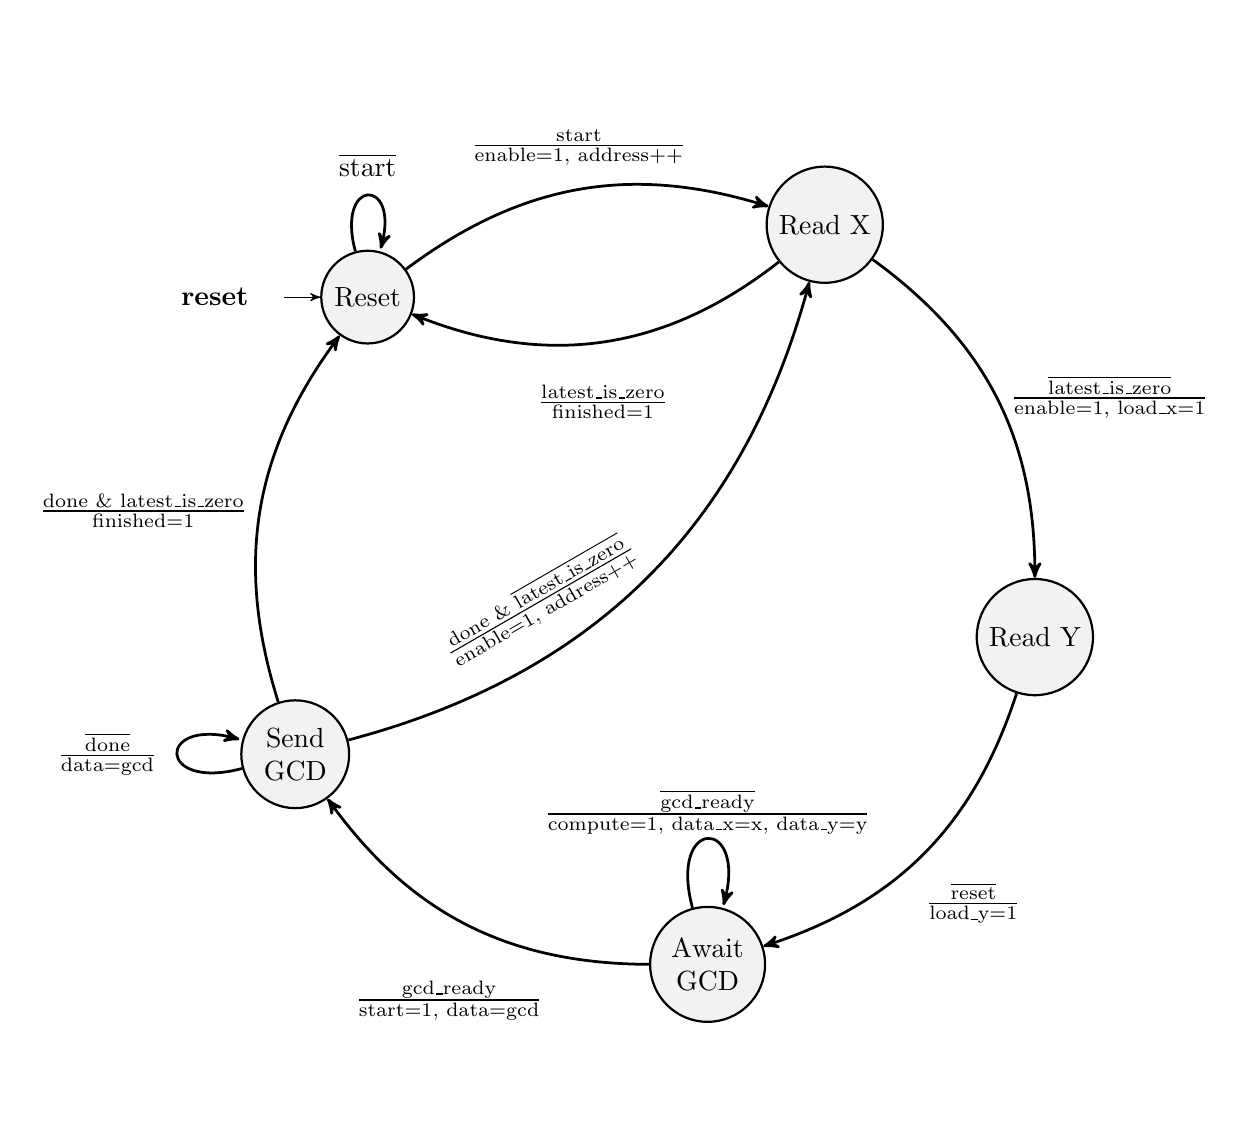
\begin{tikzpicture}[initial text=\textbf{reset}, every node/.style={circle, minimum size=1.75cm, align=center}]
	\def \curv {27}
	\node[initial, state] at ({360/5*(1-1)-45}:-5cm) (Reset) {Reset};
	\node[state] at ({360/5*(1-2)-45}:-5cm) (Read X) {Read X};
	\node[state] at ({360/5*(1-3)-45}:-5cm) (Read Y) {Read Y};
	\node[state] at ({360/5*(1-4)-45}:-5cm) (Await GCD) {Await\\ GCD};
	\node[state] at ({360/5*(1-5)-45}:-5cm) (Send GCD) {Send\\ GCD};
	\draw[->, line width=0.35mm]
		(Reset) edge[loop above] node[yshift=-0.5cm]{$\overline{\text{start}}$} (Reset)
		(Reset) edge[bend left=\curv, above] node[yshift=-1cm]{$\frac{\text{start}}{\text{enable=1, address}++}$} (Read X)
		(Read X) edge[bend left=\curv, right] node{$\frac{\overline{\text{latest\_is\_zero}}}{\text{enable=1, load\_x=1}}$} (Read Y)
		(Read X) edge[bend left, below] node[yshift=0.25cm]{$\frac{\text{latest\_is\_zero}}{\text{finished=1}}$} (Reset)
		(Read Y) edge[bend left=\curv, below right] node{$\frac{\overline{\text{reset}}}{\text{load\_y=1}}$} (Await GCD)
		(Await GCD) edge[loop above] node[yshift=-1.9cm]{$\frac{\overline{\text{gcd\_ready}}}{\text{compute=1, data\_x=x, data\_y=y}}$} (Await GCD)
		(Await GCD) edge[bend left=\curv, below left] node[xshift=0.75cm]{$\frac{\text{gcd\_ready}}{\text{start=1, data=gcd}}$} (Send GCD)
		(Send GCD) edge[loop left] node{$\frac{\overline{\text{done}}}{\text{data=gcd}}$} (Send GCD)
		(Send GCD) edge[bend right, left] node[yshift=0.5cm, rotate=30]{$\frac{\text{done \& $\overline{\text{latest\_is\_zero}}$}}{\text{enable=1, address++}}$} (Read X)
		(Send GCD) edge[bend left=\curv, left] node{$\frac{\text{done \& latest\_is\_zero}}{\text{finished=1}}$} (Reset);
\end{tikzpicture}
\caption{Top-Level Finite State Machine}
\label{fig:fsm-top-level}
\end{figure}

The most important part of this sequence of operations is that the \textbf{load\_x} and \textbf{load\_y} signals are asserted one clock cycle after their respective states. This is required because the block memory unit has a one clock cycle delay on all reading and writing operations. Beyond that, the two most important states are the \textbf{Await GCD} and \textbf{Send GCD} states. At each of these, the FSM waits indefinitely until the respective \textit{done} signals are asserted. When these are asserted is defined by the FSM's shown in \textbf{Figure~\ref{fig:fsm-gcd-calculator}} and \textbf{Figure~\ref{fig:fsm-spi}}.

The read, calculate, and send sequence is repeated for each pair of $X$ and $Y$ data read from the memory until the last read from the memory unit is evaluated to be zero. At this point the FSM terminates and this top-level \textit{done} signal (called \textbf{finished}) is asserted.

The code for this module is shown in \textbf{Listing~\ref{lst:memory-reader}}.

\subsection{GCD Calculator}
I decided to approach my GCD interaction and calculation much like the GCD wrapper from \textbf{Project \#3}. Rather than \textit{bloating} the state machine of my top-level module, I decided to create a GCD Calculator module (code shown in \textbf{Listing~\ref{lst:gcd-calculator}}) which takes both $X$ and $Y$ as parallel inputs, and when \textbf{compute} is asserted, will sequence the GCD core module. This module's FSM is shown below.

\begin{figure}[H]
\centering
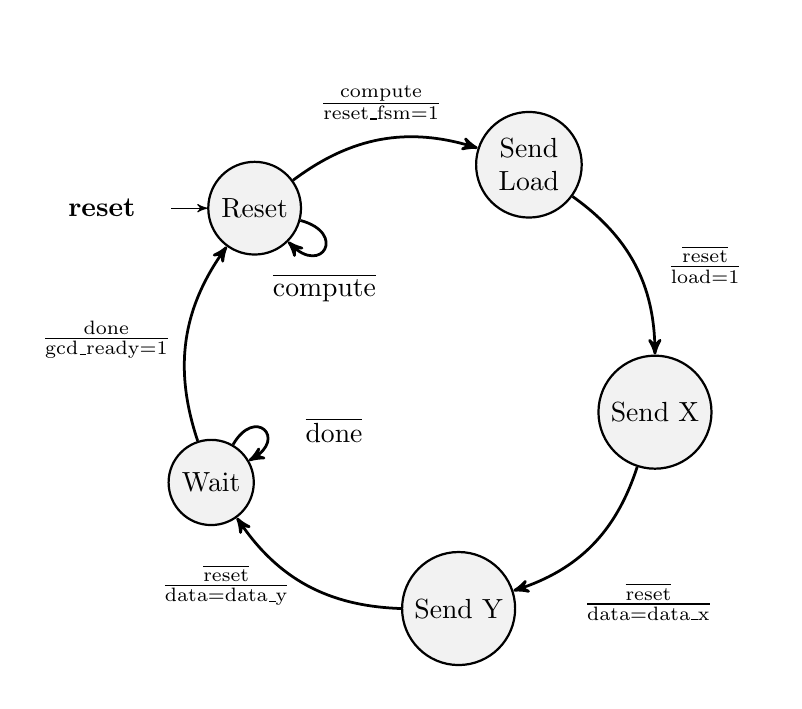
\begin{tikzpicture}[initial text=\textbf{reset}, every node/.style={circle, minimum size=1.75cm, align=center}]
	\def \curv {27}
	\node[initial, state] at ({360/5*(1-1)-45}:-3cm) (Reset) {Reset};
	\node[state] at ({360/5*(1-2)-45}:-3cm) (Send Load) {Send\\Load};
	\node[state] at ({360/5*(1-3)-45}:-3cm) (Send X) {Send X};
	\node[state] at ({360/5*(1-4)-45}:-3cm) (Send Y) {Send Y};
	\node[state] at ({360/5*(1-5)-45}:-3cm) (Wait) {Wait};
	\draw[->, line width=0.35mm]
		(Reset) edge[loop, looseness=5, in=-45, out=-15] node[yshift=-0.5cm]{$\overline{\text{compute}}$} (Reset)
		(Reset) edge[bend left=\curv, above] node[yshift=-0.5cm]{$\frac{\text{compute}}{\text{reset\_fsm=1}}$} (Send Load)
		(Send Load) edge[bend left=\curv, right] node{$\frac{\overline{\text{reset}}}{\text{load=1}}$} (Send X)
		(Send X) edge[bend left=\curv, below right] node{$\frac{\overline{\text{reset}}}{\text{data=data\_x}}$} (Send Y)
		(Send Y) edge[bend left=\curv, left] node{$\frac{\overline{\text{reset}}}{\text{data=data\_y}}$} (Wait)
		(Wait) edge[loop, looseness=5, in=30, out=60, right] node{$\overline{\text{done}}$} (Wait)
		(Wait) edge[bend left=\curv, left] node{$\frac{\text{done}}{\text{gcd\_ready=1}}$} (Reset);
\end{tikzpicture}
\caption{GCD Calculation Finite State Machine}
\label{fig:fsm-gcd-calculator}
\end{figure}

This is nearly identical to the previous project's sequencing, so not a lot of design thought had to go into this. This module blocks until the GCD Core asserts the done signal, at which point the \textbf{gcd\_result} signal is routed into the previously shown top-level module's \textbf{data} register. In order to reuse the GCD Core over and over, at the transition between the \textbf{Reset} state and the \textbf{Send Load} state the Core is reset -- however, this is unnecessary.

\subsection{SPI Module}
The majority of my design process was spent on creating the SPI module. As per my top-level module, I wanted the SPI FSM to be triggered be the internal signal \textbf{start}, and will communicate back to the reading module with the assertion of \textbf{done}.

By the end of my design, the most difficult component to implement was the SPI clock generation; which I ended up separating from my control FSM completely. I discuss my problems further in \textbf{Section~\ref{sec:tribulations}}.

\begin{figure}[H]
\centering
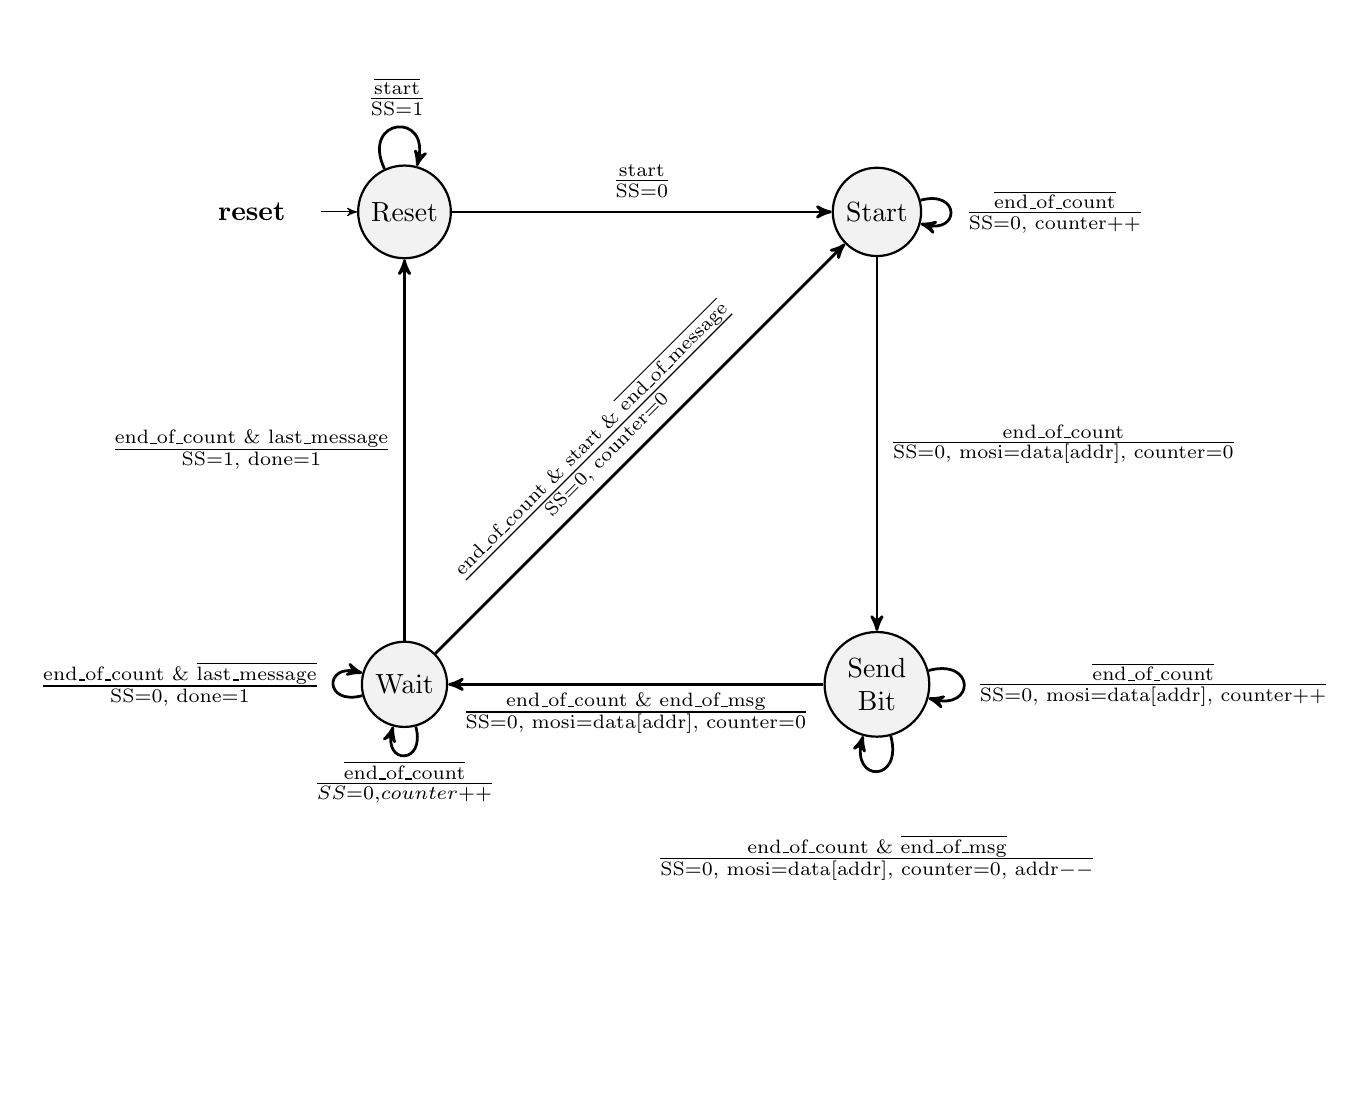
\begin{tikzpicture}[initial text=\textbf{reset}, every node/.style={circle, minimum size=1.75cm, align=center}]
	\node[state, initial] (Reset) {Reset};
	\node[state, right of=Reset] (Start) {Start};
	\node[state, below of=Start] (Send Bit) {Send\\ Bit};
	\node[state, left of=Send Bit] (Wait) {Wait};
	\draw[->, line width=0.35mm]
		(Reset) edge[loop above, in=75, out=115, looseness=4.5] node[yshift=-0.5cm]{$\frac{\overline{\text{start}}}{\text{SS=1}}$} (Reset)
		(Reset) edge[above] node[yshift=-0.5cm]{$\frac{\text{start}}{\text{SS=0}}$} (Start)
		(Start) edge[loop right, in=-15, out=15, looseness=4.5] node{$\frac{\overline{\text{end\_of\_count}}}{\text{SS=0, counter++}}$} (Start)
		(Start) edge[right] node{$\frac{\text{end\_of\_count}}{\text{SS=0, mosi=data[addr], counter=0}}$} (Send Bit)
		(Send Bit) edge[loop right, looseness=4.5] node{$\frac{\overline{\text{end\_of\_count}}}{\text{SS=0, mosi=data[addr], counter++}}$} (Send Bit)
		(Send Bit) edge[loop below, looseness=4.5] node[yshift=1.85cm]{$\frac{\text{end\_of\_count \& }\overline{\text{end\_of\_msg}}}{\text{SS=0, mosi=data[addr], counter=0, addr}--}$} (Send Bit)
		(Send Bit) edge[below] node[yshift=2cm]{$\frac{\text{end\_of\_count \& end\_of\_msg}}{\text{SS=0, mosi=data[addr], counter=0}}$} (Wait)
		(Wait) edge[loop below, looseness=4.5] node[yshift=1cm]{$\frac{\overline{\text{end\_of\_count}}}{SS=0, counter++}$} (Wait)
		(Wait) edge[loop left, looseness=4.5] node{$\frac{\text{end\_of\_count \& } \overline{\text{last\_message}}}{\text{SS=0, done=1}}$} (Wait)
		(Wait) edge[left] node{$\frac{\text{end\_of\_count \& last\_message}}{\text{SS=1, done=1}}$} (Reset)
		(Wait) edge[above] node[yshift=-1.8cm, xshift=1.3cm, rotate=45]{$\frac{\text{end\_of\_count \& start \& }\overline{\text{end\_of\_message}}}{\text{SS=0, counter=0}}$} (Start);
\end{tikzpicture}
\vspace{-3cm}
\caption{SPI Communication Finite State Machine}
\label{fig:fsm-spi}
\end{figure}

Despite being a very messy finite state machine, this is not as complicated as it might seem. Each state (excluding \textbf{Reset}) has at least one looping condition that accounts for the variable clock-slowing of the SPI bus. This is labeled as \textbf{$\overline{\text{end\_of\_count}}$}, and simply increments the counter for each clock cycle where \textbf{end\_of\_count} is not true. This functionally means that for each clock cycle that the counter is less than one-less than the desired clock delay (passed in as a parameter \textbf{clock\_scale}), nothing will change on the SPI bus -- \textit{slowing} down the communication.

At each instance of the counter reaching the entered number, the counter is reset, the address variable being used to keep track of \textit{where} in the 8-bit data line we are currently sending out over \textbf{MISO} is decremented, and then this is repeated. Once all 8 bits have been sent, the \textbf{wait} state is entered, and this state waits until start or the control signal \textbf{last\_message} is asserted. This is done to keep the slave select line \textit{low} so long as there is more data to send.

\section{Tribulations}
\label{sec:tribulations}
\subsection{Problems}
In hindsight, I should have tested each component individually. However, I ended up creating one large testbench that tested the entire integrated module. Luckily, my memory reader module and my GCD calculation module both worked as expected. The only change required between these two modules was that I did not initially account for the one-clock delay of the results from the block memory unit -- resulting in me attempting to load $X$ and $Y$ one cycle earlier than they were available. This was easily rectified by shifting the \textbf{load\_x} and \textbf{load\_y} back one state.

By far my biggest problems came from the SPI module. I began by creating the slowed clock using a counter, however I then had a much simplified FSM that was triggered by my created clock. Whether this was problematic in itself, or I simply had other fundamental errors, but I was finding that all my simulations worked as expected, except when implementing I would receive various timing errors that I could not resolve. After attempting to debug this for [what felt like] hours I ended up redoing my design completely -- deciding instead to have everything triggered by the global clock, and have the counter being utilized as a control signal.

Clock implementation ended up being much easier in this new method, but took some trial and error. I ended up implementing it as:

\begin{mdframed}[backgroundcolor=code-gray, roundcorner=10pt, innerleftmargin=25, innertopmargin=5, innerbottommargin=5]	
\begin{lstlisting}[nolol=True, caption=SPI Clock Generation, label={lst:memory-reader}]
	assign spi_clock = ~((counter > clock_scale / 2 - 1) | slave_select) & (state == send_bit); 
\end{lstlisting}
\end{mdframed}

This is a combinational assignment that sets the SPI clock high for the first half of the count (done so that the falling edge falls in the middle of the data output as opposed to the end), is only pulsing if \textbf{slave\_select} is down (we do not want the clock active while not \textit{selecting} a device), and only during the \textbf{send\_bit} state so that the clock isn't active for the required padded time at the start and end of each transmission.

The last thing I struggled with was generating the correct SPI clock frequency. I didn't realize the simulation's timescale was not representative of the board's actual frequency -- leading t me incorrectly configuring the SPI clock counter. Luckily, I choose to create the SPI module as a parameterized module so I had to simply change the parameter being used for the counter to 626.

\subsection{Tested Cases}
To validate my design, I tested different amounts of data within my block memory, between 1 and 7 pairs of data to verify the data-end verification worked as expected. I also looked at the output of my SPI communication in both the Protocol and the Logic window of Waveforms, in the cases where I spammed, held and then released, and just pressed and released the reset button. In each instance, my design behaved as expected.

\section{Simulations}
\subsection{Behavioral Simulation}
To get more clear simulations, my behavioral simulations were done with only a $\frac{1}{2}$ scaled SPI clock. All internal signals are shown in the two figures below, where I've zoomed in on just a single GCD transmission.

\begin{landscape}
\begin{figure}[H]
\centering
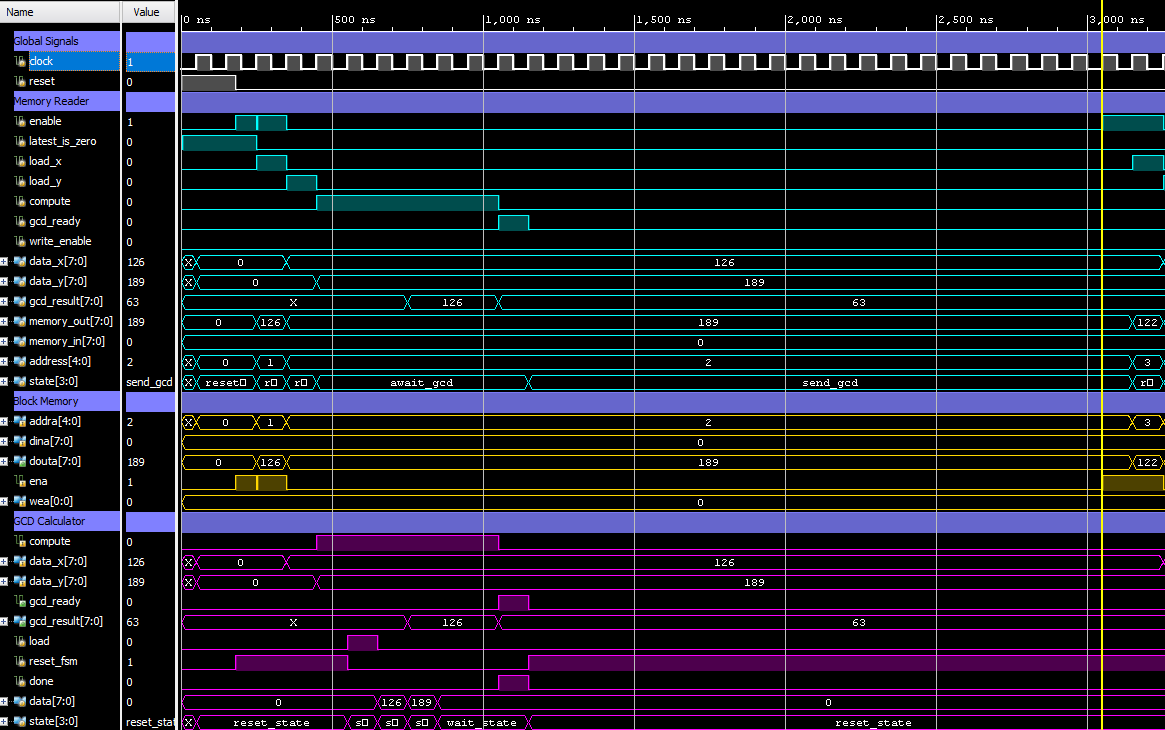
\includegraphics[width=0.80\paperheight, keepaspectratio=true]{Sources/behav-half-spi-1.PNG}
\caption{SPI Signals in Behavioral Simulation.}
\label{fig:behav-sim1}
\end{figure}

\begin{figure}[H]
\centering
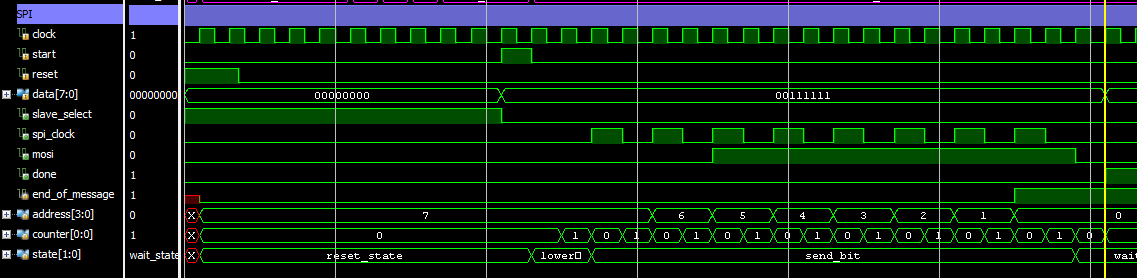
\includegraphics[width=0.85\paperheight, keepaspectratio=true]{Sources/behav-half-spi-2.PNG}
\caption{Memory Reader, Block Memory, and GCD Calculator Signals in Behavioral Simulation.}
\label{fig:behav-sim2}
\end{figure}

\subsection{Post-Synthesis Timing Simulation}
At the same clock scaling, the Post-Synthesis timing simulation shows all 6 GCD transmissions (for a preloaded block memory with 12 values).

\begin{figure}[H]
\centering
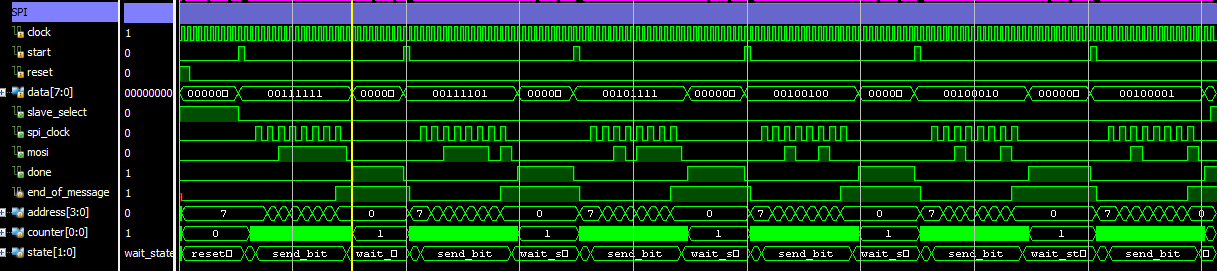
\includegraphics[width=0.85\paperheight, keepaspectratio=true]{Sources/all-spi-synth.PNG}
\caption{Post-Synthesis Timing Simulation with 6 transmissions.}
\label{fig:post-synth-sim}
\end{figure}

\subsection{Post-Implementation Timing Simulation}
The post-implementation timing simulation was done with the correct (200kHz) SPI clock. One thing to note is that the simulation appears to have \textit{blips} (on almost all signals) at transitions; however when zoomed in upon, these are not actually present.

\begin{figure}[H]
\centering
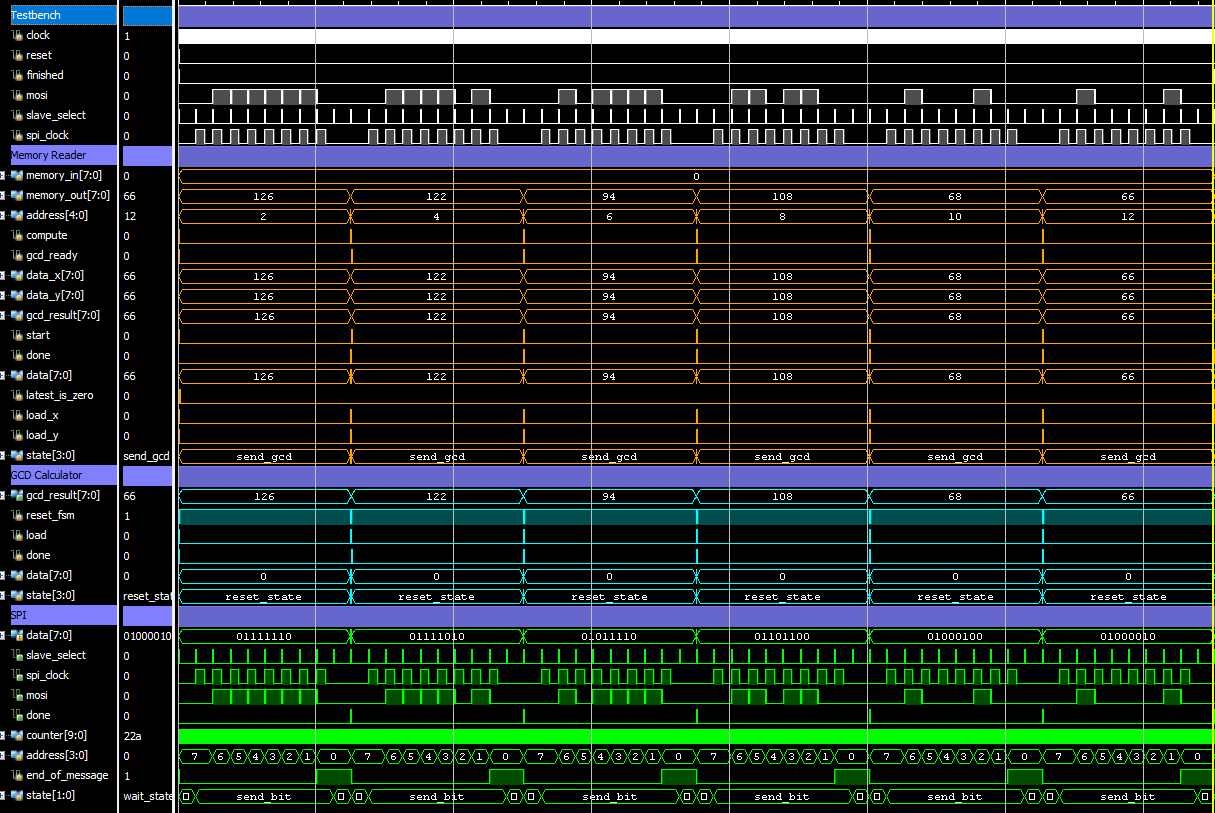
\includegraphics[width=0.85\paperheight, keepaspectratio=true]{Sources/Post-Impl-All-Signals-Sim.PNG}
\caption{Post-Implementation Timing Simulation.}
\label{fig:post-impl-sim}
\end{figure}

\subsection{WaveForms}
To verify the output of my SPI communications, I hooked up the appropriate pins on the Zybo board to the Analog Discovery, and these are the results:

\begin{figure}[H]
\centering
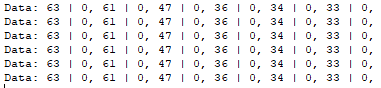
\includegraphics[width=0.55\paperheight, keepaspectratio=true]{Sources/waveforms-protocol.PNG}
\caption{WaveForms \textit{Protocol} view of the SPI output.}
\label{fig:waveforms-protocol}
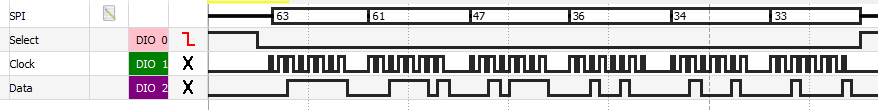
\includegraphics[width=0.85\paperheight, keepaspectratio=true]{Sources/waveforms-signals.PNG}
\caption{WaveForms \textit{Signal} view of the SPI output.}
\label{fig:waveforms-signal}
\end{figure}

In both views you can see the same data is transmitted in all instances (which is what I expected). One thing to note is that the Protocol window shows zeros between data transmissions because I believe the MISO is transmitting zeros in response -- so these can be ignored.

\end{landscape}

\section{Source Code}
\begin{mdframed}[backgroundcolor=code-gray, roundcorner=10pt, innerleftmargin=25, innertopmargin=5, innerbottommargin=5]	
\lstinputlisting[caption=Memory Reader Module, label={lst:memory-reader}]{Sources/memory_reader.sv}
\end{mdframed}

\begin{mdframed}[backgroundcolor=code-gray, roundcorner=10pt, innerleftmargin=25, innertopmargin=5, innerbottommargin=5]	
\lstinputlisting[caption=GCD Calculator Module, label={lst:gcd-calculator}]{Sources/gcd_calculator.sv}
\end{mdframed}

\begin{mdframed}[backgroundcolor=code-gray, roundcorner=10pt, innerleftmargin=25, innertopmargin=5, innerbottommargin=5]	
\lstinputlisting[caption=SPI Protocol Module, label={lst:spi}]{Sources/spi.sv}
\end{mdframed}

\begin{mdframed}[backgroundcolor=code-gray, roundcorner=10pt, innerleftmargin=25, innertopmargin=5, innerbottommargin=5]	
\lstinputlisting[caption=Hardware Wrapper, label={lst:hardware-wrapper}]{Sources/hardware_wrapper.sv}
\end{mdframed}

\end{document}